\chapter{Numerical Derivatives}\label{ch:derivatives}

When we study physics, we often investigate the change of certain quantities.  That is why basic calculus plays a major role in physics.  Evaluating the derivative of a function $f(x)$ is an ubiquitous operation in physics.  However, an analytical expression of the derivative is not always available.  Then, a numerical method must be deployed to evaluate it.  That is not only the reason we need numerical derivative.  In some cases an analytical expression of the function itself is not available.  For example, when a function is experimentally obtained by measurement, it is given as a set of numerical data, $(x_i, f_i),\, i=1, \cdots, N$.  Then, analysis of such data is always numerical.  There are many algorithms for numerical derivative.  In this chapter, we study some of well-known algorithms useful for studying physics.

Numerical methods are in general not exact and involve systematic errors.  Understanding the source of errors and their magnitude is very important.  It is possible to estimate the magnitude of expected errors based on mathematical analysis and the study of numerical error is an important part of numerical analysis.  We will investigate the degrees of errors through theory and examples.

In this section, we assume that an analytical expression of function $f(x)$ is given and that we can numerically evaluate it at any point $x$. Furthermore, we assume that the numerical error in the evaluation of the function is negligiblly small.  In other words, the main errors occur when the derivative is evaluated. 


\section{First order derivatives}\label{sec:dv-1st-order}
\begin{figure}
\centerline{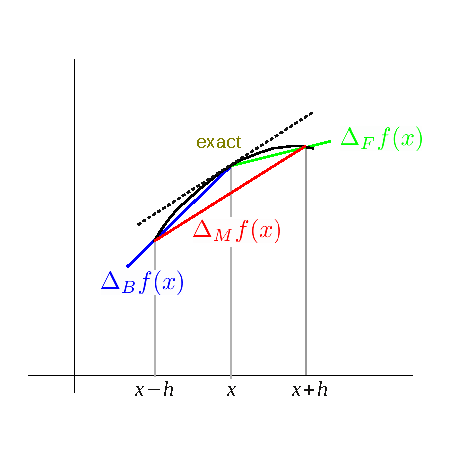
\includegraphics[width=3in]{02.derivatives/diff.pdf}}
\caption{Illustration of various numerical derivatives.  The exact derivative is the slope of the curve at $x$, which is shown as the dotted line. The forward finite difference method shown in green  underestimates the slop whereas the backward finite difference method shwon in blue overestimates it.  The mean finite different method shown in red looks very close to the exact derivative.}
\label{fig:diff}
\end{figure}
  
Let us look at the mathematical definition of derivative:
\begin{equation}\label{eq:diff_exact}
\dv{x} f(x) = \lim_{h \searrow 0} \frac{f(x+h)-f(x)}{h} = \lim_{h \searrow 0} \frac{f(x)-f(x-h)}{h}
\end{equation}
which involves limit operation which floating point calculation cannot not perform due to the quantization (See Chap. \ref{ch:numbers}).
If $h=0$ is used, we have \texttt{0/0=NaN}.
If $h$=\texttt{realmin} is used, $f(x+h)-f(x)$ is very inaccurate due to round-off error as discussed in Chapter \ref{ch:numbers}.
If  $1 \gg h >$ \texttt{realmin} is used, the both numerator and denominator are finite but the ratio is not exactly the limit.  

It is clear that direct numerical evaluation of Eq \eqref{eq:diff_exact} is not possible. 
However,  it is expected to be close to the limit if an \textit{appropriately small} value of $h$ is used.  
Based on this naive argument, we hope that the following \textit{forward finite difference} method is close to the actual derivative with a certain small value of $h$.
\begin{equation}\label{eq:diff_fwd}
\dv{x} f(x) \approx \Delta_\text{F} f(x)  \equiv \fbox{$\displaystyle \frac{f(x+h)-f(x)}{h}$}\, .
\end{equation}
where $\Delta_\text{F}$ is the forward finite difference operator. 
Similarly, we define the \textit{backward finite difference} method
\begin{equation}\label{eq:diff_bwd}
\dv{x} f(x) \approx \Delta_\text{B} f(x) \equiv \fbox{$\displaystyle \frac{f(x)-f(x-h)}{h}$}\, .
\end{equation}
where $\Delta_\text{B}$ is the backward finite difference operator. 
Unlike the exact limit (\ref{eq:diff_exact}) the forward and backward finite difference methods do not agree each other due to the finite $h$.
As illustrated in Fig. \ref{fig:diff}, one of them overestimates and the other underestimates.  

Now, we investigate how accurate the forward and backward finite difference methods are. We estimate the order of error using Taylor expansion\cite{Boas2006},
\begin{subequations}\label{eq:h.expand}
\begin{equation}
f(x+h) = f(x) + h\, f'(x) + \frac{h^2}{2} f''(x) + \frac{h^3}{3!} f^{(3)}(x) + \order{h^4}\label{eq:h+expand}
\end{equation}
\begin{equation}
f(x-h) = f(x) - h\, f'(x) + \frac{h^2}{2} f''(x) - \frac{h^3}{3!} f^{(3)}(x) + \order{h^4}\label{eq:h-expand}
\end{equation}
\end{subequations}
where $\order{h^4}$ mean that the remaining terms with $h^4$ and higher order.

Substituting the expansions \eqref{eq:h.expand} to Eqs. \eqref{eq:diff_fwd} and \eqref{eq:diff_bwd}), we find
\begin{subequations}\label{eq:derivative_error}
	\begin{equation}
    \Delta_\text{F} f(x) =  f'(x) + \frac{h}{2} f''(x) + \order{h^2}
    \end{equation}
    \begin{equation}
    \Delta_\text{B} f(x) =  f'(x) - \frac{h}{2} f''(x) + \order{h^2}  
    \end{equation}
\end{subequations}
where $f'$ and $f''$ indicate the first and second order derivatives of $f$. The leading term in the error $ \Delta_\text{F,B} f(x) - f'(x)$ is $\pm  \frac{h}{2} f''(x)$, which is the order of $h$. This means that if $h$ is small enough, the numerical methods agree with the exact derivative. However, the error decreases only linearly with $h$.  We need to remember that if $h$ is too small, the round-off error kills the accuracy.  Hence, $h$ cannot be too small.  Error at the order $h$ is in general not acceptable and these methods are not accurate enough for practical applications.

There is a better method.  Noting that the error in the forward and backward finite difference method is exactly the same in magnitude but has opposite sign, we can get rid of the error at the order of $h$.
Taking the mean of the two approximations, we obtain
\begin{equation}\label{eq:diff_mid}
\Delta_\text{M} f(x) \equiv \frac{\Delta_\text{F} f(x)+\Delta_\text{B} f(x)}{2} = \fbox{$\displaystyle\frac{f(x+h)-f(x-h)}{2h}$}\, .
\end{equation}
where $\Delta_\text{M}$ is a \textit{mean finite difference} operator.

Substituting the expansions \eqref{eq:h.expand} to \eqref{eq:diff_mid}, we find
\begin{equation}\label{eq:derivative_error_mean}
\Delta_\text{M} f(x) = f'(x) + \frac{h^2}{3!} f^{(3)}(x) + \order{h^4}
\end{equation}
Now, the error is at the order of $h^2$ which is smaller than the previous error at $h$. 
The improvement is clearly visible in Fig. \ref{fig:diff}.  

Mathematically speaking, the small error in the mean finite difference method is related to the mean value theorem\cite{mean_value_theorem} which states that there is at least one number $c$ between $a$ and $b$ such that
\begin{equation}\label{eq:mean-value-theorem}
f'(c)=\frac{f(b)-f(a)}{b-a}
\end{equation} 
Let $b=x+h$ and $a=x-h$,  the right hand side of Eq \eqref{eq:mean-value-theorem} mathces to $\Delta_\textbf{M}f(x)$.  Therefore, the mean finite different method gives the slope of the curve at some point $c$ between $x+h$ and $x-h$.  When $h$ is small, $c$ is apprximately $x$.  Then, we obtain the mean finite difference formula \eqref{eq:diff_mid}.


The mean finite element method \eqref{eq:diff_mid} is good enough for most application.
If even a higher degree of accuracy is needed, use the symmetric four-point method\cite{Zwillinger2012}
\begin{equation}
\Delta_{S4} f(x) \equiv \fbox{$\displaystyle\frac{f(x+2h) - 8 f(x+h) + 8 f(x-h) - f(x - 2h)}{12 h}$}\, .
\end{equation}
Its error is at the order of $h^4$. 

\vspace{18px}
\noindent
\exercise
Using the Taylor expansion, verify that the error of symmetric four-point method is order of $h^4$.
\vspace{18px}

How do we find an appropriate value of $h$?
Considering the definition of derivative (\ref{eq:diff_exact}), one might expect that smaller $h$ provides more accurate result. However, when $h$ is too small, the finite different methods suffer from the round-off error.  Therefore, we must choose the value of $h$  carefully, not too big and not too small. Noting that $x+h = x (1+x/h)$, it is pointless to use $h < \epsilon_\text{m}\, x$ where $\epsilon_\text{m}$ is the machine epsilon. (See Section 1.6
%%%Cross Refernce \ref{sec:epsilon} %%%
). Example \ref{ex:derivatives} illustrates that the finite difference method fails when $h$ is too small. 


\bigskip
\begin{example}[Round-off errors in finite difference methods]\label{ex:derivatives}
Let's numerically evaluate the derivative of $f(x)=\displaystyle\frac{1}{3}x^3$ at $x=1$ and compare the results with the exact value.
The analytic form of derivative is $f'(x)=x^2$ and thus the exact value is $f'(1)=1$.  Program \ref{prog:derivative} computes the derivative using the forward, backward and mean finite difference methods for
$h=1, 0.1, 0.01, \cdots, 10^{-19}$.  The error is measured by $\delta = |f'(1)-\Delta f(1)|$.  The results are plotted in Fig.
\ref{fig:derivatives}.  The error of forward and backward methods is almost the same and decreases in the same way as $h$.  However, the improvement stop at $h \sim 10^{-8}$ and the error increases for smaller $h$ due to the round-off error. The best answer is obtained with $h=10^{-8}$. The mean difference method shows much better result.  The error decreases with $h^2$.  The best value is obtained at $h=10^{-5}$ and the result is better than the best value obtained by the forward or backward method.  It is quite clear that the mean difference method is much better than the two others.
\begin{figure}[t]
\centerline{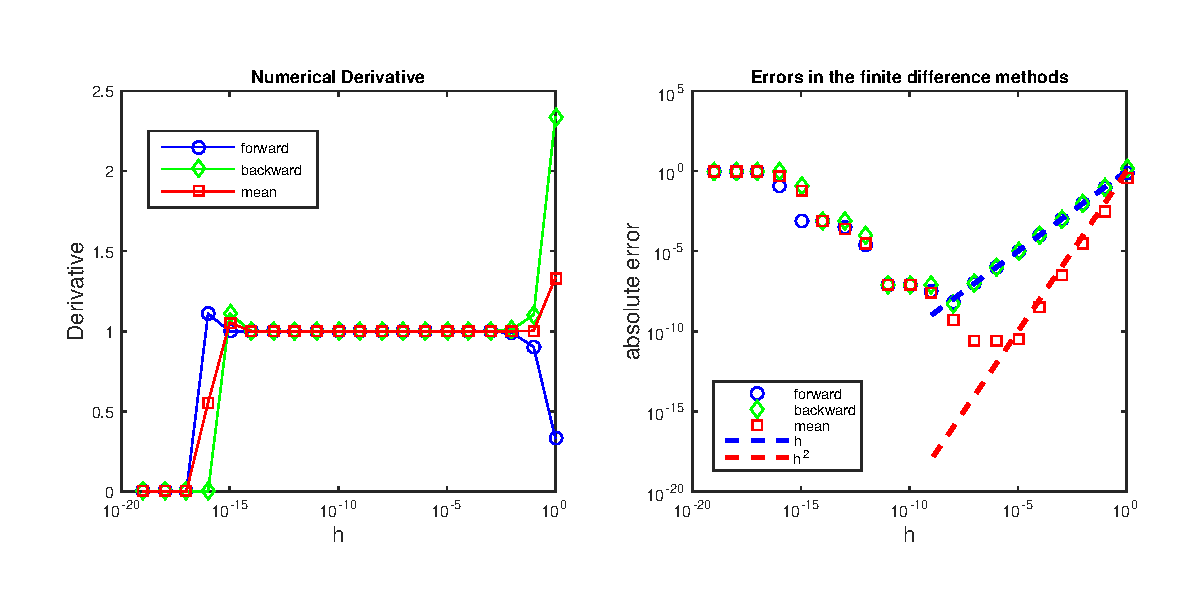
\includegraphics[width=6.0in]{02.derivatives/derivative-plot.pdf}}
\caption{Output of Example \ref{ex:derivatives}.  The left panel shows numerical derivatives for wide ranges of $h$.  As $h$ decreases from $h=1$ to $h=0.01$, the derivative converges to 1 (at least in our eyes). As $h$ further decreases, the values of all methods remain the same until $h \approx \epsilon_\text{m}$.  Below it, the derivative abruptly goes to 0.  The numerical method fails due to round-off error. To see more details, the right panel plots the error. As $h$ decreases, the error of the forward and backward finite difference methods decreases in the same way as $h$ until $h \approx 10^{-8}$ but the error increases when $h$ is further reduced.  The mean finite difference method shows smaller error than the two other methods and the error decreases as $h^2$ up to $h \sim 10^{-5}$.  The best result is given by the mean finite difference method with $h \approx 10^{-5}$.}
\label{fig:derivatives}
\end{figure}
\end{example}
\bigskip

In practice, we don't know the actual error and therefore we cannot use a plot like the right panel of Fig. \ref{fig:derivatives} to find an appropriate value for $h$.  However, the left panel of Fig. \ref{fig:derivatives} shows that the numerical derivative approaches a certain value and the output does not change much when $h$ is smaller than a certain value until it hits the limit of round-off error.
Suppose that we calculate the derivative using $h$ and $h'=h/2$.  We expect that the output is more accurate with $h'$ than $h$. Using Eq. (\ref{eq:derivative_error_mean}), the change of the mean finite difference is given by
\begin{equation}
\left | \Delta_\text{M} f(x) - \Delta'_\text{M} f(x) \right | = \frac{|f^{(3)}|}{3!} \frac{3}{4} h^2 = \frac{3}{4} \times  \left [ \text{error in } \Delta_\text{M} f(x) \right ]
\end{equation}
which suggests that the error is estimated by
\begin{equation}
\text{Error in }\Delta_M f(x) \approx  \left | \Delta_\text{M} f(x) - \Delta'_\text{M} f(x) \right |  
\end{equation}. 
Note that the exact value of $f'(x)$ is not needed to find the error.
Now we have an algorithm to find numerical derivative with a desired accuracy using this error estimate.  

\bigskip

\begin{myalgobox}
\Algorithm{Numerical derivative with tolerance}\label{algo:derivative-auto}

\medskip
\begin{enumerate}
\item Set a value of \textit{tolerance} (allowed error).
\item Set a reference step size $h_1$ and evaluate a reference derivative $g_1 = \Delta_\text{M} f(x)$ using $h_1$.
\item Set a new step size $h_2=h_1/2$ and evaluate a new derivative $g_2 = \Delta_\text{M} f(x)$ using $h_2$.
\item Evaluate error $\delta = |g_2-g_1|$.
\item If $\delta < \text{tolerance}$, $g_2$ is the desired result.  Stop the loop.
\item If not, let $g_1=g_2$ and $h_1=h_2$ (previous $g_2$ and $h_2$ are now the reference).
\item Go back to Step 3.
\end{enumerate}
\end{myalgobox}


\bigskip\noindent
Here the absolute error is used.  We can also use a relative error $\left |\displaystyle \frac{g_2 - g_1}{g_1} \right |$ instead. Then, the tolerance specifies a desired relative error. 

\begin{example}[Automatic adjustment of the step size $h$.]
We numerically evaluate the derivative of  $f(x)=\displaystyle\frac{1}{3}x^3$ at $x=1$ again.  This time, we do not specify the step length $h$. Instead we specify a tolerance and the program will automatically find an appropriate $h$ for the given tolerance.  Program \ref{prog:derivative-auto} implements Algorithm \ref{algo:derivative-auto}.  When the tolerance is 0.001, we obtain the following output.
It appears that $h=0.03125$ is good enough for this problem.  



\begin{mybox}
\small
\begin{verbatim}
Enter tolerance =0.001
    h       derivative            error
 5.000e-01 1.0833333333e+00 2.5000000000e-01
 2.500e-01 1.0208333333e+00 6.2500000000e-02
 1.250e-01 1.0052083333e+00 1.5625000000e-02
 6.250e-02 1.0013020833e+00 3.9062500000e-03
 3.125e-02 1.0003255208e+00 9.7656250000e-04
Tolerance is OK.
\end{verbatim}
\normalsize
\end{mybox}
\end{example}

\vspace{18px}
\noindent
\exercise
Evaluate of the derivative of $\sin(x)$ at $x=\pi/4$ using the mean finite difference method.  The first three digits of the answer should be correct.

\vspace{18px}

\noindent
\section{Second order derivatives}

We can evaluated the second order derivative using the mean value method twice.
First, we pretend that the first order derivative is given. Using the mean value method with step size $h/2$, we obtain
\begin{equation}
f''(x) \approx \Delta_M f'(x) = \frac{f'(x+\frac{h}{2})-f'(x-\frac{h}{2})}{h}
\end{equation}
Then, we replace the first order derivatives with approximated ones using the mean value method again.
\begin{subequations}
\begin{equation}
f'(x+\frac{h}{2}) \rightarrow \Delta_M f(x+\frac{h}{2}) = \frac{f(x+h)-f(x)}{h}
\end{equation}
\begin{equation}
f'(x-\frac{h}{2}) \rightarrow \Delta_M f(x-\frac{h}{2}) = \frac{f(x)-f(x-h)}{h}.
\end{equation}
\end{subequations}
The result is
\begin{equation}\label{eq:diff2-s3}
f''(x) \approx \Delta^{(2)}_M f(x) \equiv \fbox{$\displaystyle\frac{f(x+h)+f(x-h)-2f(x)}{h^2}$}.
\end{equation}
where $\Delta^{(2)}_M$ is the second order mean finite difference operator.
Substituting Eqs. (\ref{eq:h+expand}) and (\ref{eq:h-expand}) into (\ref{eq:diff2-s3}), we find that the error of this approximation is order of $h^2$.  

\vspace{18px}
\noindent
\exercise
The second order derivative of $\sin(x)$ is $-\sin(x)$.  Evaluate the second order derivative of $\sin(x)$ at $x=2 n \pi / N$ where $n=0, 1, \cdots, N$.  Use $N=100$ and plot the result. Verify that it is $-\sin(x)$ at least within the accuracy of the numerical method.

\vspace{18px}

If a higher accuracy is needed, use the symmetric five-point method
\begin{equation}\label{eq:diff2-s5}
f''(x) \approx \Delta^{(2)}_{S5} f(x) \equiv \fbox{$\displaystyle\frac{-f(x+2h) + 16 f(x+h) - 30 f(x) + 16 f(x-h) - f(x-2 h)}{12 h^2}$}
\end{equation}
whose error is the order of $h^4$.\cite{diff2}

\vspace{18px}
\noindent
\exercise
Using the Taylor expansion, verify that the error of symmetric five-point method is order of $h^4$.

\vspace{18px}



\noindent
\section*{Problems}
\addcontentsline{toc}{section}{\protect\numberline{}Problems}

\begin{enumerate}[labelwidth=0.5cm,labelindent=0cm,leftmargin=*,label=\bfseries \thechapter.\arabic*,align=left]
	
\item Evaluate the first order derivative of $\sin(x)$ for interval $(0,2\pi)$ with tolerance 0.0001. What value of $h$ is needed to satisfy the tolerance?  Compare the numerical derivative with the exact one $\cos(x)$ and check if the tolerance is indeed satisfied. 
\item Evaluate the second order derivative of $f(x)=\displaystyle\frac{1}{12} x^4$ at $x=1$ using $h=1, 0.1, 0.01, \cdots, 10^{-10}$.
Plot the error as a function of $h$. Plot also the theoretical error $h^2$ for the three-point method \eqref{eq:diff2-s3}. [Optional: Try also the five-point method \eqref{eq:diff2-s5} and check how the error increases.  Unexpectedly, the larger $h$ gives better answer.  The symmetric five-point formula takes into account up to the fourth order derivative. The fifth and higher order derivative of $x^4$ vanishes and thus the five-point formula is theoretically exact for $x^4$.  Nevertheless, you encounter numerical errors due to the loss of significance.  Therefore, the larger $h$ is better for this particular function.  Try the same calculation with $f(x)=\displaystyle\frac{1}{20}x^5$. You will see the usual error profile.]
%
\end{enumerate}

\vspace{1 in}
\bigskip
\noindent
\section*{MATLAB Source Codes}
\addcontentsline{toc}{section}{\protect\numberline{}MATLAB Source Codes}
\setcounter{program}{0}

\bigskip
\noindent
\program\label{prog:derivative}

\footnotesize
\begin{verbatim}
%**************************************************************************
%*     Example  2.1                                                       *
%*     filename: ch02pr01.m                                               *
%*     program listing number: 2.1                                        *
%*                                                                        *
%*  This program evaluates the derivative of a given function func(x)     *
%*  at x=1 using the three finite difference methods.                     *
%*  Errors in forward, backward and mean value methods are plotted.       *
%*                                                                        *
%*     Programed by Ryoichi Kawai for Computational Physics Course.       *
%*     Last modification:  12/25/2013.                                    *
%**************************************************************************
clear all;

% define the function
func = @(x) x^3/3;

x=1;  % the point at which derivative is evaluated.
imax=20; % number of different displacements

% title and headers
display('Absolute Errors')
fprintf('%4s %16s %18s %20s\n','h','forward','backward','mean value')

for i=1:imax
    
    % Small displacement
    h(i)=10^(-i+1);
    
    % Evaluation of numerical derivative
    d_f(i)=(func(x+h(i))-func(x))/h(i); % Forward diffrence
    d_b(i)=(func(x)-func(x-h(i)))/h(i); % Backward diffrence
    d_m(i)=(func(x+h(i))-func(x-h(i)))/(2*h(i)); % Mean value
    
    % Errors
    err_f(i)=abs(1-d_f(i));
    err_b(i)=abs(1-d_b(i));
    err_m(i)=abs(1-d_m(i));
    
    % Display the errors
    fprintf('%6.1e %18.10e %18.10e %18.10e\n',...
            h(i),err_f(i),err_b(i),err_m(i));
end

hh = h.*h; % h^2 (the error of the mean value formula is order of h^2)

% Plot data
subplot(1,2,1)  % left panel
q=semilogx(h(1:imax),d_b(1:imax),'-o',...
    h(1:imax),d_f(1:imax),'-d',...
    h(1:imax),d_m(1:imax),'-s');
title('Numerical Derivative');
xlabel('h','fontsize',14);
ylabel('Derivative','fontsize',14);
set(q(1),'Color','blue');
set(q(2),'Color','green');
set(q(3),'Color','red');    
legend(q,{'forward','backward','mean'});
legend(q,'Location','NorthWest');

subplot(1,2,2) % right panel
p=loglog(h(1:imax),err_b(1:imax),'o',...
    h(1:imax),err_f(1:imax),'d',...
    h(1:imax),err_m(1:imax),'s',...
    h(1:imax/2),h(1:imax/2),'--',h(1:imax/2),hh(1:imax/2),'--');
title('Errors in the finite difference methods');
xlabel('h','fontsize',14);
ylabel('absolute error','fontsize',14);
set(p(1),'Color','blue');
set(p(2),'Color','green');
set(p(3),'Color','red');
set(p(4),'Color','blue','LineWidth',2);
set(p(5),'Color','red','LineWidth',2);
legend(p,{'forward','backward','mean','h','h^2'});
legend(p,'Location','SouthWest');
\end{verbatim}
\normalsize

\ruleend

\bigskip\noindent
\program
\label{prog:derivative-auto}

\footnotesize
\begin{verbatim}
%**************************************************************************
%*  Example  2.2                                                          *
%*  filename: ch02pr02.m                                                  *
%*  program listing number: 2.2                                           *
%*                                                                        *
%*  This program evaluates the derivative of a given function func(x)     *
%*  at x=1 using the mean finite difference method with the accuracy      *
%*  specified by tolerance.                                               *
%*                                                                        *
%*     Programed by Ryoichi Kawai for Computational Physics Course.       *
%*     Last modification:  01/01/2017.                                    *
%**************************************************************************
clear all;

% define the function
func = @(x) x^3/3;

% Read tolerance from keyboard.
tol=input('Enter tolerance =');  % 

x=1;  % point where derivative is evaluated
h=1; % initial interval
diff_old=(func(x+h)-func(x-h))/(2*h); % initial numerical derivative

% any value bigger than tol is OK here.
delta = tol+1;

fprintf('%5s %18s %14s\n','h','derivative','error')

% Repeat until error is smaller than tolerance.
while delta>tol
    h=h/2;
    diff_new=(func(x+h)-func(x-h))/(2*h);
    delta=abs(diff_new-diff_old);
    fprintf('%10.3e %16.10e %16.10e\n',h,diff_new,delta)
    diff_old=diff_new;
end
fprintf('Tolerance is OK.\n')


\end{verbatim}
\normalsize

\ruleend

\bigskip
\noindent
\section*{Python Source Codes}
\addcontentsline{toc}{section}{\protect\numberline{}Python Source Codes}
\setcounter{program}{0}

\bigskip
\noindent
\program

\footnotesize
\begin{verbatim}
#!/usr/bin/env python3
# -*- coding: utf-8 -*-
"""
%**************************************************************************
%*  Example  2.1                                                          *
%*  filename: ch02pr01.py                                                 *
%*  program listing number: 2.1                                           *
%*                                                                        *
%*  This program evaluates the derivative of a given function func(x)     *
%*  at x=1 using the three finite difference methods.                     *
%*  Errors in forward, backward and mean value methods are plotted.       *
%*                                                                        *
%*     Programed by Ryoichi Kawai for Computational Physics Course.       *
%*     Last modification:  01/01/2017.                                    *
%**************************************************************************
"""
import numpy as np
import matplotlib.pyplot as plt
       
def func(x):
    return x**3/3

def main():
    x=1.0
    imax=20
    h=np.zeros(imax)
    d_f=np.zeros(imax)
    d_b=np.zeros(imax)
    d_m=np.zeros(imax)
    err_f=np.zeros(imax)
    err_b=np.zeros(imax)
    err_m=np.zeros(imax)
    i=0
    print("{0:^62}".format('Absolute Errors'))
    print("{0:^6} {1:^18} {2:^18} {3:^20}"
          .format('h','forward','backward','mean value'))
    while(i<imax):
    # Small displacement
        h[i]=10**(-i)
    
    # Evaluation of numerical derivative
        d_f[i]=(func(x+h[i])-func(x))/h[i] # Forward diffrence
        d_b[i]=(func(x)-func(x-h[i]))/h[i] # Backward diffrence
        d_m[i]=(func(x+h[i])-func(x-h[i]))/(2*h[i]) # Mean value

    # Errors
        err_f[i]=abs(1.-d_f[i])
        err_b[i]=abs(1.-d_b[i])
        err_m[i]=abs(1.-d_m[i])
        print("{0:6.1e} {1:18.10e} {2:18.10e} {3:18.10e}"
              .format(h[i],err_f[i],err_b[i],err_m[i]))
        i=i+1

    # Plot data
    plt.ioff()
    plt.figure(figsize=(12,5))
    plt.subplot(1,2,1)
    plt.semilogx(h,d_f, '--ob', label='forward')
    plt.semilogx(h,d_b, '--dg', label='backword')
    plt.semilogx(h,d_m, '--sr', label='mean')
    plt.legend(loc=2)
    plt.xlabel('h')
    plt.ylabel('Derivative')
    
    plt.subplot(1,2,2)
    plt.loglog(h,err_f, '--ob', label='forward')
    plt.loglog(h,err_b, '--dg', label='backword')
    plt.loglog(h,err_m, '--sr', label='mean')
    plt.legend(loc=3)
    plt.xlabel('h')
    plt.ylabel('Absolute error')
    plt.show()
      
if __name__ == "__main__":
    main()
\end{verbatim}
\normalsize

   \ruleend 

\footnotesize
\begin{verbatim}
    #!/usr/bin/env python3
    # -*- coding: utf-8 -*-
    """
    %**************************************************************************
    %*  Example  2.2                                                          *
    %*  filename: ch02pr02.py                                                 *
    %*  program listing number: 2.2                                           *
    %*                                                                        *
    %*  This program evaluates the derivative of a given function func(x)     *
    %*  at x=1 using the mean finite difference method with the accuracy      *
    %*  specified by tolerance.                                               *
    %*                                                                        *
    %*     Programed by Ryoichi Kawai for Computational Physics Course.       *
    %*     Last modification:  01/01/2017.                                    *
    %**************************************************************************
    """
    
    import numpy as np
    import matplotlib.pyplot as plt
           
    def func(x):  # define a function
        return x**3/3
    
    def main():
        tol=input("Enter tolerance =")  # Read a tolerabce from the console
        tol=np.float(tol)
        x=1.0
        h=1.0   # initial interval
        diff_old=(func(x+h)-func(x-h))/(2.0*h)  #  derivative first try
        delta=np.finfo(float).max  # any value bigger than tol is OK.
    
        print("{0:^10} {1:^16} {2:^16}"
              .format('h','derivative','error'))
        while (delta>tol):
            h=h/2.0
            diff_new=(func(x+h)-func(x-h))/(2.0*h)  # improved derivative
            delta=np.abs(diff_new-diff_old)
            print("{0:10.3e} {1:16.10e} {2:16.10e}"
                  .format(h,diff_new,delta))
            diff_old=diff_new
            
        print("Tolerance is OK.")
        
    if __name__ == "__main__":
        main()
\end{verbatim}
        
\normalsize
\vfill
%\chapbibliography
\bibliographystyle{unsrt}
\bibliography{compphys}

